% jupiter-data-refinement-illustration.tex

% !TEX program = pdflatex
\documentclass[tikz]{standalone}
% jupiter-illustration-preamble.tex

\usepackage{tikz}
\usetikzlibrary{shapes, positioning, arrows.meta, calc, backgrounds, fit}

\def\hdist{1.8}
\def\vdist{2.0}
\tikzset{node distance = \vdist and \hdist}

\tikzset{every lower node part/.style = {red}}
\newcommand{\statesplit}[4]{% #1: state upper label; #2: state lower label; #3: position; #4: name
  \node (#4) [circle split, draw, minimum size = 6mm, text width = 10mm, align = center, #3, font = \Large]
  {
    $#1$
    \nodepart{lower}
    $#2$
  };
}

\newcommand{\rectsplit}[2]{% #1: state upper label; #2: state lower label
  \node [draw, rectangle split, rectangle split parts = 2, 
    align = center, font = \Large]
  {
    #1
    \nodepart{two}
    \textcolor{red}{#2}
  };
}

\newcommand{\transition}[4][]{% #2: start state; #3: end state; #4: transition label; #1: transition label position (optional)
  \draw[>=Stealth, ->] (#2) to node (#2to#3) [rectangle, draw, above = 2pt, sloped, #1, font = \small] {$#4$} (#3);
}

\newcommand{\set}[1]{\{#1\}}
\newcommand{\ins}[2]{\textsc{Ins}(#1,#2)}
\newcommand{\del}[2]{\textsc{Del}(#2)}
% \newcommand{\del}[2]{\textsc{Del}(#1,#2)}


\usetikzlibrary{arrows.meta}

\begin{document}
\begin{tikzpicture}[bg/.style = {rectangle, draw, very thick}, 
    refine/.style = {>=Stealth, ->, very thick, #1}]

  % absjupiter-c3-4
  \node (absj) [label = {[font = \Huge] above : AbsJupiter}] 
    {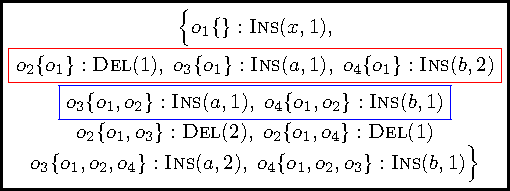
\includegraphics[scale = 2.00]{absjupiter-c3-set}};

  % cjupiter-c3-4
  \node (cj) [below = 3.0cm of absj, 
    label = {[font = \Huge, below = 15pt] below : CJupiter}] 
    {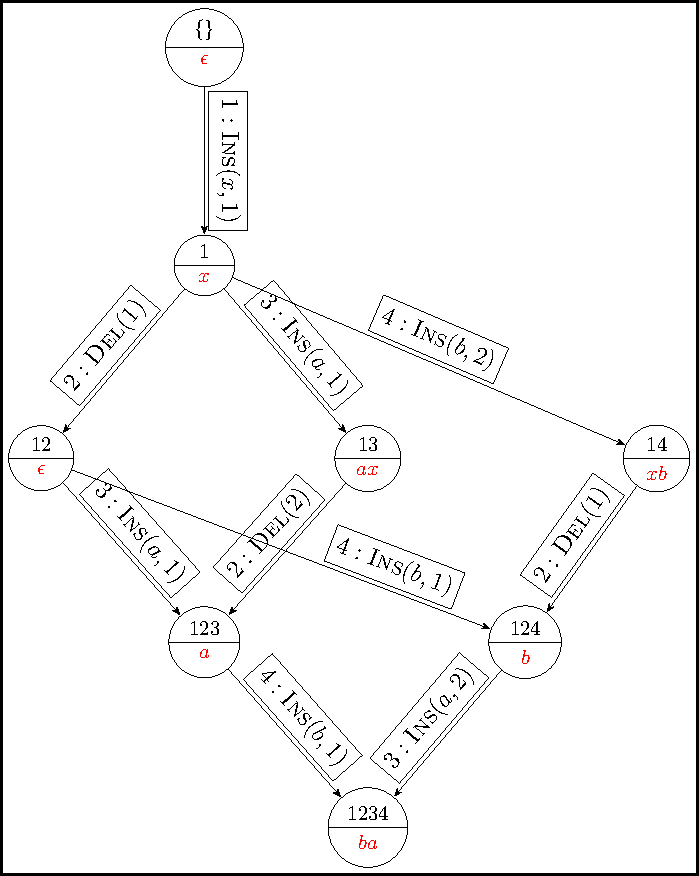
\includegraphics[scale = 1.50]{cjupiter-c3-nary-digraph}};

  % xjupiter-c3-4
  \node (xj) [right = 1.5cm of cj, 
    label = {[font = \Huge, below = 15pt] below : XJupiter}]
    {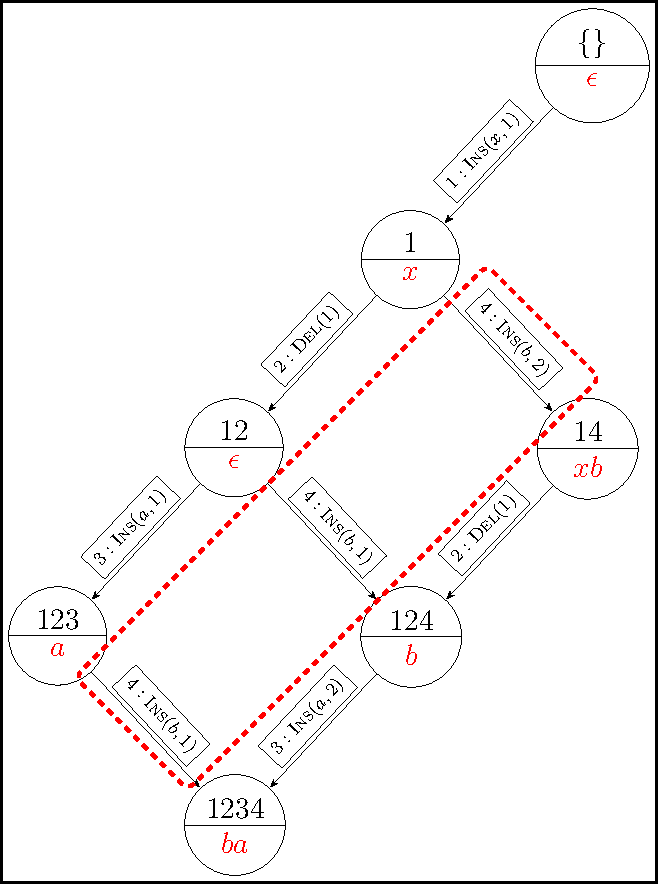
\includegraphics[scale = 1.50]{xjupiter-c3-2d-digraph}};

  % ajupiter-c3-4
  \node (aj) [above = 3.0cm of xj, 
    label = {[font = \Huge] above : AJupiter}] 
    {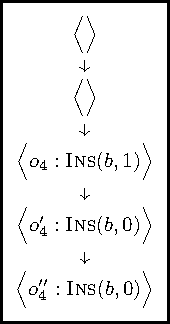
\includegraphics[scale = 2.00]{ajupiter-c3-buffer}};

  % absj -> cj
  \draw [refine] (absj) 
    to node [font = \Huge, align = center] 
    {organized into $n$-ary digraph}
    (cj);

  % cj -> xj
  \draw [refine = {bend right = 20}] (cj.south) 
    to node [above = 10pt, font = \Huge, align = center] 
    {optimization at clients}
    (xj.south);

  % xj -> aj
  \draw [refine] (xj) 
    to node [font = \Huge, align = center] 
    {local dimension at clients \\ remote dimension at the server}
    (aj);
\end{tikzpicture}
\end{document}